\documentclass[../main.tex]{subfiles}
\begin{document}
\chapter{Platonic Solids}
\section{Platonic and Dual Solids}
Amazingly, while there are infinitely many regular 2D polygons.
In 3D there are only five \textit{platonic solids}.
\begin{definition}[Platonic Solid]
  A convex polyhedron $X \subseteq \R^3$ is a \textit{platonic solid} if:
  \begin{itemize}
    \item Every face is a regular $n$-gon for some $n$.
    \item $G = \Isom (X)$ acts transitively on the faces.
      That is, there exists a symmetry that takes any face to any other face.
    \item If $x \in X$ is the midpoint of a face $\Stab_G(x) \cong D_{2n}$
  \end{itemize}
\end{definition}
\begin{theoremlike}[The 5 Platonic Solids]{Fact}
  There are, up to similarity, 5 platonic solids:
  \begin{enumerate}
    \item The \textit{tetrahedron} -- 4 triangular faces, 4 vertices
    \item The \textit{cube} -- 6 square faces, 8 vertices
    \item The \textit{octahedron} -- 8 triangular faces, 6 vertices
    \item The \textit{dodecahedron} -- 12 pentagonal faces, 20 vertices
    \item The \textit{icosahedron} -- 20 triangular faces, 12 vertices
  \end{enumerate}
\end{theoremlike}

\begin{definition}[Dual Solids]
  Two solids $X, Y$ are \textit{dual} if $Y$ can be constructed from $X$ by putting vertices in the centres of each face, and then joining vertices in adjacent faces by edges.
\end{definition}
\begin{example}[Cube and Octahedron]
  The cube and the octahedron are \textit{dual}.
  \begin{center}
  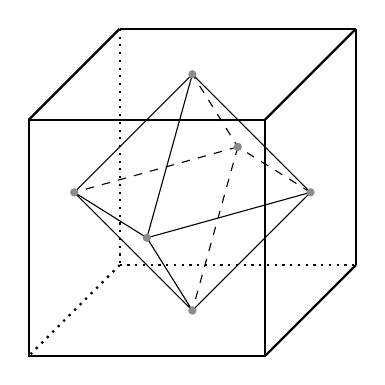
\begin{tikzpicture}[scale=3]
  \coordinate (A) at (0,0,0);
  \coordinate (B) at (1,0,0);
  \coordinate (C) at (1,1,0);
  \coordinate (D) at (0,1,0);
  \coordinate (E) at (0,0,1);
  \coordinate (F) at (1,0,1);
  \coordinate (G) at (1,1,1);
  \coordinate (H) at (0,1,1);

  \draw[thick, dotted] (A) -- (B);
  \draw[thick] (B) -- (C);
  \draw[thick] (C) -- (D);
  \draw[thick, dotted] (D) -- (A);
  \draw[thick] (E) -- (F) -- (G) -- (H) -- cycle;
  \draw[thick, dotted] (A)--(E);
  \draw[thick] (B) -- (F);
  \draw[thick] (C) -- (G);
  \draw[thick] (D) -- (H);

  \coordinate (O1) at (0.5,0.5,0);
  \coordinate (O2) at (0.5,0.5,1);
  \coordinate (O3) at (0.5,0,0.5);
  \coordinate (O4) at (0.5,1,0.5);
  \coordinate (O5) at (0,0.5,0.5);
  \coordinate (O6) at (1,0.5,0.5);

  \draw[dashed] (O6) -- (O1) -- (O4);
  \draw[dashed] (O1) -- (O5);
  \draw[dashed] (O1) -- (O3);
  \draw (O4) -- (O2) -- (O5) -- cycle;
  \draw (O4) -- (O6) -- (O2);
  \draw (O5) -- (O3) -- (O2);
  \draw (O3) -- (O6);

  \foreach \p in {O1,O2,O3,O4,O5,O6} \fill[gray!90] (\p) circle (0.5pt);
  \end{tikzpicture}
  \end{center}
  If we take either of these and carry out this construction, we get the other of the pair.
\end{example}
\begin{remark}
  We can get hints to what solids are dual by looking for solids where the number of faces of one matches the number of vertices of the other and vice versa.

  This is a necessary condition for two solids to be dual.
  In this case we have:
  \begin{itemize}
    \item The tetrahedron is dual to itself.
    \item The cube and octahedron and dual.
    \item The dodecahedron and icosahedron are dual.
  \end{itemize}
\end{remark}

If $X$ and $Y$ are dual, then $\Isom X \cong \Isom Y$.
This means that we only have 3 symmetry groups to identify up to isomorphism for all 5 platonic solids.
\section{Symmetries of a Tetrahedron}
\subsection{Full Symmetry Group}
\begin{center}
\tdplotsetmaincoords{340}{45}
\begin{tikzpicture}[scale=1.5, tdplot_main_coords]
\coordinate (A) at (1, 1, 1);
\coordinate (B) at (1, -1, -1);
\coordinate (C) at (-1, 1, -1);
\coordinate (D) at (-1, -1, 1);

\draw[thick] (A) -- (B) -- (C) -- (A);
\draw[thick, dashed] (A) -- (D);
\draw[thick] (B) -- (D) -- (C);
\end{tikzpicture}
\end{center}
Let $G = \Isom(\text{Tetrahedron})$.
By definition, $G$ acts transitively on the faces and each stabiliser is isomorphic to $D_6$.
So Orbit-Stabiliser gives:
\[
  |G| = |\Stab_G(x)||Gx| = 6 \times 4 = 24
\]
Furthermore, the action of $G$ on the 4 vertices defines a homomorphism:
\[
  \theta: G \to S_4
\]
We now wish to prove that $\theta$ is injective.
Suppose $\theta(g) = e$, so $g$ is an isometry that fixes 4 points that are not all coplanar.
Thus, by the 4-point lemma (\cref{threePointLemma}), we have $g = \id$.
So $\ker \theta$ is trivial.
Therefore, by \cref{surjectiveInjectiveProp}, $\theta$ is injective as claimed so we may identify $G$ with a subgroup of $S_4$.
However both $G$ and $S_4$ have size 24, so $G \cong S_4$.
\subsection{Rotational Symmetries}
We can also identify the group of \textit{rotational symmetries} of a tetrahedron:
\[
  G_0 = G \cap \SO(3)
\]
where the tetrahedron is centered on the origin.
\begin{lemma}[Uniqueness of $A_n$]
  If $H \leq S_n$ and $|S_n : H| = 2$, then $H = A_n$.
\end{lemma}
\begin{proof}
  Since $|S_n : H| = 2$, by \cref{quotientExamples}, we see that $H \lhd S_n$ and $S_n / H \cong C_2$.
  We therefore have a homomorphism:
  \[
    \theta: S_n \to C_2 = \{\pm 1\}
  \]
  with $\ker \theta = H$.
  This must be surjective as otherwise $\ker \theta = H = S_n$ which contradicts $|S_n : H| = 2$.
  So we must have some element that is mapped to $-1$.
  Since transpositions generate $S_n$ (\cref{transpositionsGenerate}), we can write the image of each element as a product of the images of transpositions.
  This must be $-1$ for some element of $S_n$ so there must be some transposition $\tau_0$ such that $\theta(\tau_0) = -1$.

  We also know that all transpositions are conjugate (\cref{conjugateCycles}).
  Consider any transposition $\tau = \sigma \tau_0 \sigma^{-1}$ for some $\sigma \in S_n$:
  \begin{align*}
    \theta(\tau) &= \theta(\sigma \tau_0 \sigma^{-1}) \\
                 &= \theta(\sigma)\theta(\tau_0)\theta(\sigma^{-1}) \\
                 &= \theta(\sigma)(\theta(\sigma))^{-1}\theta(\tau_0) \text{ as $C_2$ is abelian}\\
                 &= \theta(\tau_0) \\
                 &= - 1
  \end{align*}
  So $\theta$ acts like the sign homomorphism on all transpositions.
  Again, since transpositions generate $S_n$, this means that $\theta = \sign$.
  Thus, $H = \ker \theta = \ker(\sign) = A_n$.
\end{proof}
Since $G_0 = G \cap SO(3) = \ker(\det: G \to C_2)$:
\[
  |G: G_0| = |\im(\det: G \to C_2)| \leq 2
\]
We know the cube has reflectional symmetries, thus we must have $|G: G_0| = 2$.
Therefore we can apply the above lemma, so $G_0 \cong A_4$.
\section{Symmetries of the Cube and Octahedron}
Let $G  = \Isom(\text{Cube})$.
We have already found the size of this group in \cref{cubeSymmetries} using Orbit-Stabiliser so we know $|G| = 48$.

\subsection{Rotational Symmetries}
In particular, the index two rotational subgroup $G_0$ has:
\[
  |G_0| = \frac{48}{2} = 24
\]
When identifying the symmetries of a tetrahedron, we considered the action of $G$ on a small set that was manageable to analyse.
If we tried to use $S_8$ here, it would be very difficult as $|S_8| = 40320$.
We could think about the action on the midpoints of the faces (or equivalently the vertices of an octahedron), however $|S_6| = 720$ which is still fairly large.

However, in Sheet 2 Q7, we saw that $G$ acts on the set of four long diagonals of the cube.
So we obtain a homomorphism:
\[
  \theta: G_0 \to S_4
\]
Since $|G_0| = |S_4| = 24$, to show injectivity, it is sufficient to show surjectivity.
\begin{proof}
  Since transpositions generate $S_4$, it suffices to show that all transpositions are contained in $\im \theta$.
  To do this, we first need to find a rotational symmetry that swaps two only two diagonals.
  \begin{center}
  \tdplotsetmaincoords{80}{125}
  \begin{tikzpicture}[scale=3, tdplot_main_coords]
  \coordinate (A) at (0,0,0);
  \coordinate (B) at (1,0,0);
  \coordinate (C) at (1,1,0);
  \coordinate (D) at (0,1,0);
  \coordinate (E) at (0,0,1);
  \coordinate (F) at (1,0,1);
  \coordinate (G) at (1,1,1);
  \coordinate (H) at (0,1,1);

  \draw[thick, dotted] (A)--(B);
  \draw[thick] (B)--(C);
  \draw[thick] (C)--(D);
  \draw[thick, dotted] (D)--(A);
  \draw[thick] (E)--(F)--(G)--(H)--cycle;
  \draw[thick, dotted] (A)--(E);
  \draw[thick] (B)--(F);
  \draw[thick] (C)--(G);
  \draw[thick] (D)--(H);


  \draw (A) node[below] {$A_1$} -- (G) node[above] {$A_2$};
  \draw (B) node[below] {$B_1$} -- (H) node[above] {$B_2$};
  \draw (C) node[below] {$C_1$} -- (E) node[above] {$C_2$};
  \draw (D) node[below] {$D_1$} -- (F) node[above] {$D_2$};

  \coordinate (M1) at (1.2, -0.2, 0.5);
  \coordinate (M2) at (-0.2, 1.2, 0.5);
  \draw[dashed] (M1) -- (M2) node[right] {Rotation Axis};
  \end{tikzpicture}
  \end{center}

  If we perform rotation by $\pi$ about the axis through the midpoints of opposite edges we see the following:
  \begin{itemize}
    \item $A_1$ and $A_2$ get swapped so the diagonal $A$ is preserved.
    \item Similarly, $C_1$ and $C_2$ are swapped so the diagonal $C$ is preserved.
    \item $D_2$ and $B_1$ are swapped and $D_1$ and $B_2$ are swapped, so the diagonals $D$ and $B$ are swapped.
  \end{itemize}
  Since this rotation only swaps two diagonals, this rotation must be mapped to a transposition under $\theta$.
  The cube has 6 pairs of opposite edges so we can get 6 unique transpositions this way.
  There are $\binom{4}{2} = 6$ transpositions in $S_4$, so $\im \theta = S_4$ as claimed.
\end{proof}
Hence, by comparing sizes, $G_0 \cong S_4$.

\subsection{Full Symmetry Group}
\label{cubeFullSymmetry}
Consider the element $-I \in G$:
\begin{itemize}
  \item $- I \notin G_0$ commutes with everything in $G_0$.
  \item $|G_0||\langle -I \rangle| = 24 \times 2 = |G|$.
  \item $G_0 \cap \langle -I \rangle = \{\id\}$ as $-I$ is not a rotation.
  \item $|-I| = 2$ so $\langle -I \rangle \cong C_2$.
\end{itemize}
We can therefore apply the Direct Product Theorem (\cref{directProductTheorem}) to yield:
\[
  G \cong S_4 \times C_2
\]
\section{Symmetries of the Dodecahedron and Icosahedron}
\nonexaminable
Let $G = \Isom(\text{Dodecahedron})$ and let $G_0$ be the rotational subgroup of index two.
Since a face has an orbit of size 12 and a stabiliser of size 10, we can apply Orbit-Stabiliser:
\[
  |G| = |\Stab_G(x)||Gx| = 12 \times 10 = 120 \implies |G_0| = 60
\]
By drawing diagonals on the faces, we may inscribe 5 different cubes into the dodecahedron:
\clearpage
\begin{figure}[t]
  \centering
  \includegraphics[width=6cm]{figures/dodecahedron.png}
  \label{dodecahedronFig}
  \caption{Dodecahedron with 5 inscribed cubes.\\\footnotesize\url{https://www.chiark.greenend.org.uk/~sgtatham/polypics/dodec-cubes.html}}
\end{figure}
Since the 5 cubes are built symmetrically from the geometry of the dodecahedron, $G$ acts on them.
\subsection{Rotational Symmetries}
The above action leads to a homomorphism:
\[
  \theta: G_0 \to S_5
\]
From the diagram, we see that if we rotate about the axis through an opposite pair of vertices by angle $\frac{2\pi}{3}$, then we get a 3-cycle.
For example, for the vertex closest to the viewpoint, rotation preserves the yellow and green cubes but cycles the blue, black, and red cubes and is thus a three cycle.

There are 10 different pairs of opposite pairs of vertices so we get 10 pairs of 3-cycles and their inverses for a total of 20 3-cycles.
We saw in \cref{conjugacyA5} that there are 20 3-cycles in $S_5$ so all the three cycles of $S_5$ are in $\im \theta$.
\begin{lemma}
  If $X \leq A_5$ is set of 3-cycles in $A_5$, then $A_5 = \langle X \rangle$.
\end{lemma}
\begin{proof}
  By Sheet 4 Q2, the subgroup generated by a conjugacy class is a normal subgroup, thus:
  \[
    \langle X \rangle \lhd A_5
  \]
  From \cref{A5Simple}, we know that $A_5$ is simple, so $\langle X \rangle$ is either $A_5$ or $1$.
  However, there are certainly nontrivial elements in $\langle X \rangle$, thus $\langle X \rangle = A_5$.
\end{proof}
In summary, if $X$ is the set of 3-cycles, we have seen that:
\[
  X \subseteq \im \theta \text{ and } \langle X \rangle = A_5 \leq \im \theta
\]
Therefore:
\[
  60 = |G_0| \geq |\im \theta| \geq |A_5| = 60
\]
Since this is a chain of inequalities starting an with equality at either end, all the inequalities must be equalities and thus $|G| = |\im \theta| = |A_5|$.
Therefore $\theta$ is an isomorphism between $G_0$ and $A_5$ so $G_0 \cong A_5$.
\subsection{Full Symmetry Group}
Similarly to with the cube and octahedron in \cref{cubeFullSymmetry}, $-I \in G$ is a symmetry of the dodecahedron that commutes with everything in $G_0$ so we have:
\[
  G \cong A_5 \times C_2
\]
by the Direct Product Theorem (\cref{directProductTheorem}).
\end{document}
